\documentclass{article}
\usepackage{ae,aecompl}
\usepackage{todonotes}
\usepackage{chngcntr}
\usepackage{tikz-cd}
\usepackage{graphicx}
\graphicspath{ {./images/}}
\usepackage[all,cmtip]{xy}
\usepackage{amsmath, amscd}
\usepackage{amsthm}
\usepackage{amssymb}
\usepackage{amsfonts}
\usepackage{bm}
\usepackage{qsymbols}
\usepackage{latexsym}
\usepackage{mathrsfs}
\usepackage{mathtools}
\usepackage{cite}
\usepackage{color}
\usepackage{url}
\usepackage{enumerate}
\usepackage{verbatim}
\usepackage[draft=false, colorlinks=true]{hyperref}
\usepackage{pdfpages}
\usepackage[margin=1.2in]{geometry}
\usepackage{IEEEtrantools}

\usepackage{fancyhdr}


\usepackage[nameinlink]{cleveref}


\DeclareMathOperator*{\ac}{accept}
\DeclareMathOperator*{\amax}{argmax}
\DeclareMathOperator*{\amin}{argmin}
\DeclareMathOperator*{\Aut}{Aut}
\newcommand {\al}{{\alpha}}
\newcommand {\abs}[1]{{\left\lvert#1\right\rvert}}
\newcommand {\A}{{\mathcal{A}}}
\newcommand {\AM}{{\mathrm{AM}}}
\newcommand {\AMp}{{\AM_{p}^{X}\!(\Ri_\w)}}
\newcommand {\B}{{\mathcal{B}}}
\DeclareMathOperator*{\Be}{Bern}
\newcommand {\Br}{{\dot{B}}}
\newcommand {\Ba}{{\mathfrak{B}}}
\newcommand {\C}{{\mathbb C}}
\newcommand {\ce}{\mathrm{c}}
\newcommand {\Ce}{\mathrm{C}}
\newcommand {\Cc}{\mathrm{C_{c}}}
\newcommand {\Ccinf}{\mathrm{C_{c}^{\infty}}}
\DeclareMathOperator{\cov}{Cov}
\DeclareMathOperator{\DEV}{DEV}
\newcommand {\Di}{{\mathbb D}}
\newcommand {\dom}{\mathrm{dom}}
\newcommand{\dist}{\stackrel{\mathrm{dist}}{=}}
\newcommand {\ud}{\mathrm{d}}
\newcommand {\ue}{\mathrm{e}}
\newcommand {\eps}{\varepsilon}
\newcommand {\veps}{\varepsilon}
\newcommand {\vrho}{{\varrho}}
\newcommand {\E}{{\mathbb{E}}}
\newcommand {\Ec}{{\mathcal{E}}}
\newcommand {\Ell}{L}
\newcommand {\Ellp}{{L_{p}[0,1]}}
\newcommand {\Ellpprime}{{L_{p'}([0,1])}}
\newcommand {\Ellq}{{L_{q}([0,1])}}
\newcommand {\Ellqprime}{{L_{q'}([0,1])}}
\newcommand {\Ellr}{L^{r}}
\newcommand {\Ellone}{{L_{1}([0,1])}}
\newcommand{\Elltwo}{{L_{2}([0,1])}}
\newcommand{\Ellinfty}{L^{\infty}}
\newcommand{\Ellinftyc}{L_{\mathrm{c}}^{\infty}}
\newcommand{\exb}[1]{\exp\left\{#1\right\}}
\DeclareMathOperator*{\Ext}{Ext}
\newcommand{\F}{{\mathcal{F}}}
\newcommand{\Fe}{{\mathbb{F}}}
\newcommand{\G}{{\mathcal{G}}}
\newcommand{\HF}{\mathcal{H}_{\text{FIO}}^{1}(\Rd)}
\newcommand{\Hr}{H}
\newcommand{\HT}{\mathcal{H}}
\newcommand{\ui}{\mathrm{i}}
\newcommand{\I}{{I}}
\newcommand{\J}{{\mathcal{J}}}
\newcommand{\id}{{\mathrm{id}}}
\newcommand{\iid}{\stackrel{\mathclap{\normalfont\mbox{iid}}}{\sim}}
\newcommand{\im}{{\text{im }}}
\newcommand{\ind}{{\perp\!\!\!\perp}}
\DeclareMathOperator*{\Int}{int}
\newcommand{\intx}{{\overline{\int_{X}}}}
\newcommand{\inte}{{\overline{\int_{\E}}}}
\newcommand{\la}{\lambda}
\newcommand{\rb}{\rangle}
\newcommand{\lb}{{\langle}}
\newcommand{\La}{\Lambda}
\newcommand{\calL}{{\mathcal{L}}}
\newcommand{\lp}{{\mathcal{L}}^{p}}
\newcommand{\lpo}{{\overline{\mathcal{L}}^{p}\!}}
\newcommand{\Lpo}{{\overline{\Ell}^{p}\!}}
\newcommand{\M}{{\mathbf{M}}}
\newcommand{\Ma}{{\mathcal{M}}}
\newcommand{\N}{{{\mathbb N}}}
\newcommand{\Na}{{{\mathcal{N}}}}
\newcommand{\norm}[1]{\left\|#1\right\|}
\newcommand{\normm}[1]{{\left\vert\kern-0.25ex\left\vert\kern-0.25ex\left\vert #1 
    \right\vert\kern-0.25ex\right\vert\kern-0.25ex\right\vert}}
\newcommand{\Om}{{{\Omega}}}
\newcommand{\one}{{{\bf 1}}}
\newcommand{\pic}{\text{Pic }}
\newcommand{\ph}{{\varphi}}
\newcommand{\Pa}{{\mathbb{P}}}
\newcommand{\Po}{{\mathcal{P}}}
\newcommand{\Q}{{\mathbb{Q}}}
\newcommand{\R}{{\mathbb R}}
\newcommand{\Rd}{{\mathbb{R}^{d}}}
\DeclareMathOperator{\rej}{reject }
\newcommand{\Rn}{{\mathbb{R}^{n}}}
\newcommand{\cR}{{\mathcal{R}}}
\newcommand{\Rad}{{\mathrm{Rad}}}
\newcommand{\ran}{{\mathrm{ran}}}
\newcommand{\Ri}{{\mathrm{R}}}
\newcommand{\supp}{{\mathrm{supp}}}
\newcommand{\Se}{\mathrm{S}}
\newcommand{\Sp}{S^{*}(\Rn)}
\newcommand{\St}{{\mathrm{St}}}
\newcommand{\Sw}{\mathcal{S}}
\newcommand{\T}{{\mathcal{T}}}
\newcommand{\ta}{{\theta}}
\newcommand{\Ta}{{\Theta}}
\newcommand{\topp}{\stackrel{p}{\to}}
\newcommand{\todd}{\stackrel{d}{\to}}
\newcommand{\toL}[1]{\stackrel{L^{#1}}{\to}} 
\newcommand{\toas}{\stackrel{a.s.}{\to}}
\DeclareMathOperator{\V}{Var}
\newcommand {\w}{{\omega}}
\newcommand {\W}{{\mathrm{W}}}
\newcommand {\Wnp}{\text{$\mathrm{W}$\textsuperscript{$n,\!p$}}}
\newcommand {\Wnpeq}{\text{$\mathrm{W}$\textsuperscript{$n\!,\!p$}}}
\newcommand {\Wonep}{\text{$\mathrm{W}$\textsuperscript{$1,\!p$}}}
\newcommand {\Wonepeq}{\text{$\mathrm{W}$\textsuperscript{$1\!,\!p$}}}
\newcommand {\X}{{\mathcal{X}}}
\newcommand {\Z}{{{\mathbb Z}}}
\newcommand {\Za}{{\mathcal{Z}}}
\newcommand {\Zd}{{\Z[\sqrt{d}]}}
\newcommand {\vanish}[1]{\relax}

\newcommand {\wh}{\widehat}
\newcommand {\wt}{\widetilde}
\newcommand {\red}{\color{red}}

% Distributions
\newcommand{\normal}{\mathsf{N}}
\newcommand{\poi}{\mathsf{Poisson}}
\newcommand{\bern}{\mathsf{Bernoulli}}
\newcommand{\bin}{\mathsf{Binomal}}
\newcommand{\multi}{\mathsf{Multinomial}}
\newcommand{\Exp}{\mathsf{Exp}}



% put your command and environment definitions here




% some theorem environments
% remove "[theorem]" if you do not want them to use the same number sequence


  \newtheorem{thrm}{Theorem}
  \newtheorem{lemma}{Lemma}
  \newtheorem{prop}{Proposition}
  \newtheorem{cor}{Corollary}

  \newtheorem{conj}{Conjecture}
  \renewcommand{\theconj}{\Alph{conj}}  % numbered A, B, C etc

  \theoremstyle{definition}
  \newtheorem{defn}{Definition}
  \newtheorem{ex}{Example}
  \newtheorem{exs}{Examples}
  \newtheorem{question}{Question}
  \newtheorem{remark}{Remark}
  \newtheorem{notn}{Notation}
  \newtheorem{exer}{Exercise}

\DeclareMathOperator{\sgn}{sign}


\title{STATS305A - Lecture 15}
\author{John Duchi\\ Scribed by Michael Howes}
\date{11/11/21}

\pagestyle{fancy}
\fancyhf{}
\rhead{STATS305A - Lecture 15}
\lhead{11/11/21}
\rfoot{Page \thepage}

\begin{document}
\maketitle
\tableofcontents
\section{Overview}
Today we will be talking about advanced predictive methods in regression. Namely
\begin{itemize}
    \item Boosting with: \begin{itemize}
        \item Decision stumps.
        \item Decision trees.
    \end{itemize}
    \item Locally weighted regression.
\end{itemize}
\section{Boosting}
Motivation: We don't know apriori what the ``right'' features, scalings, etc are. 

Idea: iteratively add ``best'' features into a given model.

Setting: We have a collection of potential features
\[\Phi = \{ \phi : \X \to \R\}.\]
\subsection{Decision stumps}
A common choice of $\Phi$ is the set of \emph{decision stumps} $\phi : \R^d \to \{\pm 1\}$ where 
\begin{align*}
    \phi(x) &= \begin{cases}
        1    & \text{if } x_j \ge \tau,\\
        -1  & \text{if } x_j < \tau.
    \end{cases}\\
    &=\sgn(x_j - \tau).
\end{align*}
Our basic question is given a sample $(x_i,y_i)_{i=1}^n$ such that $x_i \in \R^d$ and $y_i \in \R$, how can we fit the the best decision stump? Our idea is to find the stump which is most correlted with the response $y$. Define
\[\wh{c}(\tau,j) := \sum_{i=1}^n y_i \sgn(x_{ij}-\tau),\]
which is the coreelation between a stump for feature $j$ and the response $(y_i)_{i=1}^n$. We thus wish to choose a pair $(j,\tau) \in [d]\times \R$ that maximizes $\abs{\wh{c}(j,\tau)}$. How do we do this? The key observation is that we should sort our $x_i$ for each coordinate $j$. For a fixed $j$ write
\[x_{(1),j} \le x_{(2),j} \le \ldots \le x_{(n),j}. \]
Note that $\wh{c}(\tau,j)$ is constant on the intervals $\tau \in (-\infty, x_{(1),j})$, $\tau \in [x_{(i),j},x_{(i+1),j})$ and $\tau \in [x_{(n),j},\infty)$. This is because the signs $\sgn(x_{ij}-\tau)$ are constant on said intervals (see picture). Thus we only need to test $n+1$ values of $\tau$ for each $j$. These values correspond to the red lines. 

\begin{center}
    
    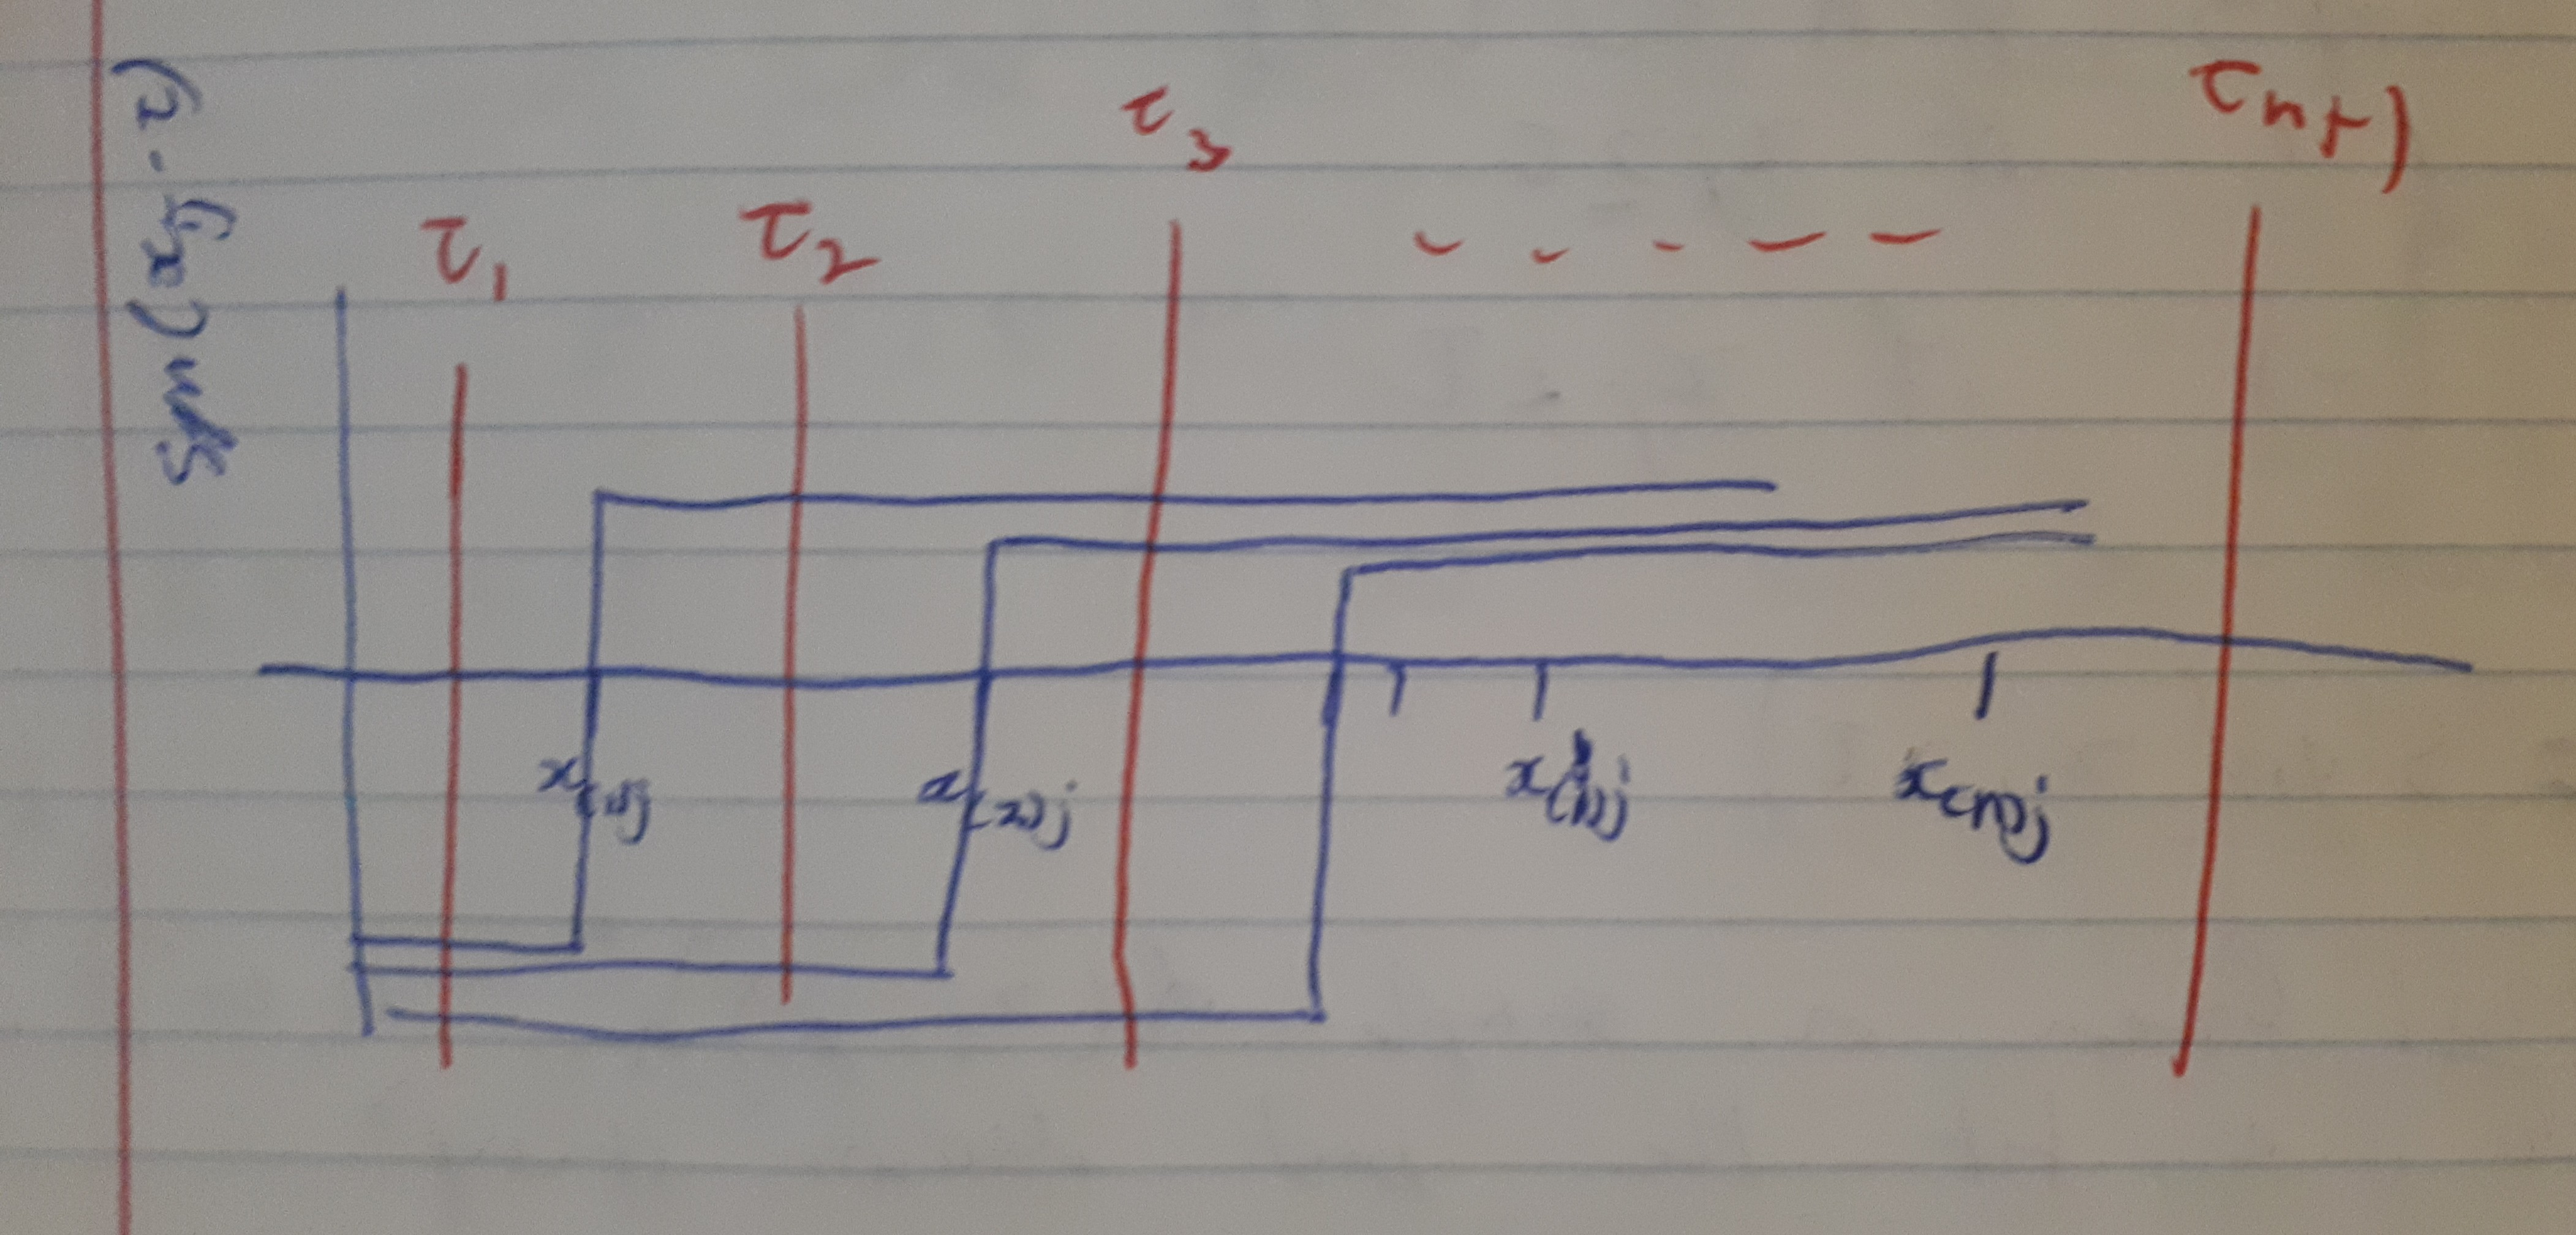
\includegraphics[width = 0.7\textwidth]{11_11_P01.jpg}
\end{center}

We thus have the following algorithm for finding the best decision stump. For each coordinate sort $x_{ij}$ (this takes time $O(dn\log(n))$). Evaluate $y^T\sgn(x^{(j)}-\tau)$ for the $n+1$ values of $\tau$ where $X= [x^{(1)},\ldots, x^{(d)}]$. Since there are $d$ coordinatex and $n+1$ thresholds we need to caclulate $d(n+1)$ inner products in $\R^n$ giving us a total run time of \[O(d(n+1)n+dn\log(n))=O(dn^2).\] 
But with another idea we can reduce this run time. Suppose our thresholds from sorting $x^{(j)}$ are $\tau_1 < \tau_2 < \ldots < \tau_{n+1}$. Then 
\begin{align*}
    \wh{c}(\tau_1,j) &= y^T\one \\
    \wh{c}(\tau_2,j) &= y^T\one - 2y_{(1)}\\
    &= \wh{c}(\tau_1,j) + 2y_{(1)}\\
    \vdots ~&~~~~~ \vdots \\
    \wh{c}(\tau_{k+1},j) &= \wh{c}(\tau_k,j)-2y_{(k)}\\
    \vdots ~&~~~~~ \vdots \\
    \wh{c}(\tau_{n+1},j) &= \wh{c}(\tau_k,n)-2y_{(n)}\\
    &=-y^T\one,
\end{align*}
where $(1), (2),\ldots, (n)$ are the indices from sorting $x^{(j)}$. That is,
\[x^{(j)}_{(1)} \le x^{(j)}_{(2)} \le \ldots \le x^{(j)}_{(n)}.  \]
Thus we can calculate the $n$ inner products for coordinate $j$ in linear time. Thus we can find the most correlated decision stump in time \[O(dn\log(n)).\]
\subsection{Boosting iteration}
Let 
\[X = \begin{bmatrix}
    x_1^T\\ \vdots\\ x_n^T
\end{bmatrix}, \]
be our matrix of features. Suppose that at iteration $k$ we have a model $M_k(X)$ given by 
\[M_k(X) = [\phi_1(X), \phi_2(X),\ldots, \phi_k(X)],\]
where 
\[ \phi_j(X) = \begin{bmatrix}
    \phi_j(x_1)\\ \vdots \\ \phi_j(x_n)
\end{bmatrix} \in \R^n.\]
Also let 
\[\wh{\beta}^k = \amin_b \norm{M_k(X)-y}_2^2.\]
How do we add a feature to this model? Define,
\[R_k(\ta,\phi) = \frac{1}{2}\norm{M_k(X)\wh{\beta}^k + \ta \phi(X)-y}_2^2,\]
where $\ta \in \R$ and $\phi \in \Phi$ and 
\[\phi(X) = \begin{bmatrix}
    \phi(x_1)\\ \vdots \\ \phi(x_n)
\end{bmatrix} \in \R^n. \]
The quantity $R_k(\ta,\phi)$ is the residual sum of squares when we add a feature $\phi : \X \to \R$ and a parameter $\ta \in \R$ to our model. Note that $\wh{\beta}^k$ is fixed. If we define 
\[y^k = y-M_k(X)\wh{\beta}^k, \]
then 
\[R_k(\ta,\phi) = \frac{1}{2}\norm{y^k - \ta \phi(X)}_2^2. \]
Thus we can think of minimizing $R_k(\ta,\phi)$ as a one-dimensional regression where we fit $y^k$ onto $\phi(X)$. Our goal is to choose $\phi$ that minimizes or approximately minimizes $R_k(\ta,\phi)$. There are two methods for choosing this $\phi$.
\begin{itemize}
    \item \underline{Version 1}: We choose $\phi$ to maximize $\abs{\frac{\partial}{\partial \ta}R_k(\ta,\phi)|_{\ta = 0}}$. That is, we do an approximation and choose the value of $\phi$ which gives us the best marginal benefit of adding $\phi$.
    \item \underline{Version 2}: We choose $\phi$ to minimize $\inf_{\ta} R_k(\ta,\phi)$. Such a $\phi$ would be an exact solution to our minimization problem.
\end{itemize}

Let's do some calculations for both these methods. Note that 
\[\frac{\partial}{\partial \ta} R_k(\ta,\phi) = \ta \norm{\phi(X)}_2^2 - \phi(X)^T y^k. \]
At $\ta = 0$ we thus have 
\[\frac{\partial}{\partial \ta} R_k(\ta,\phi)\Big|_{\ta = 0} = -\phi(X)^T y^k. \]
Thus we choose $\phi$ to maximize the aboslute value of the correlation between $\phi(X)$ and $y^k$. Note that for decision stumps we have seen how to do this efficiently.

We'll now turn to the second version. Define
\[R^*_k(\phi) = \inf_\ta R_k(\ta,\phi). \]
We wish to choose $\phi$ that minimizes $R^*_k(\phi)$. Recall that
\[R_k(\ta,\phi) = \frac{1}{2}\norm{y^k - \ta \phi(X)}_2^2.\]
Thus the infimum in $R^*_k$ is obtained and it is obtained at 
\[ \ta_\phi = \frac{\phi(X)^T y_k}{\norm{\phi(X)}_2^2}.\]
Thus 
\begin{align*}
    R^*_k(\phi) &= R_k(\ta_\phi,\phi)\\
    &= \frac{1}{2}\norm{y^k - \frac{\phi(X)^Ty^k}{\norm{\phi(X)}^2_2}\phi(X)}_2^2\\
    &= \frac{1}{2}\norm{y^k}_2^2 - \frac{1}{2}\norm{\frac{\phi(X)^Ty^k}{\norm{\phi(X)}^2_2}\phi(X)}_2^2\\
    &=\frac{1}{2}\norm{y^k}_2^2 - \frac{1}{2}\frac{(\phi(X)^T y^k)^2}{\norm{\phi(X)}_2^2}.
\end{align*}
Thus $R^*_k(\phi)$ is also maximized when the absolute value of the correlation between $\phi(X)$ and $y^k$ is maximized. Just like with the previous version/method. With both methods we choose $\phi_{k+1}$ to be the element of $\Phi$ that is most correlated with $y^k$.

After  choosing $\phi_{k+1}$ set 
\[M_{k+1}(X) = [\phi_1(X),\ldots, \phi_{k+1}(X)],\]
and
\[\wh{\beta}_{k+1} = \amin_{b \in \R^{k+1}}\norm{M_{k+1}(X)b-y}_2^2.\]
This is an example of \emph{fully-corrective boosting}. In standing boosting we do the following:
\begin{align*}
    \wh{\ta}_{k+1} &= \amin_{\ta \in \R}R_k(\ta,\phi_{k+1})\\
    &= \amin_{\ta \in \R}\frac{1}{2}\norm{y^k - \ta \phi_{k+1}(X)}_2^2\\
    &= \frac{\phi_{k+1}(X)^T y^k}{\norm{\phi_{k+1}(X)}_2^2},
\end{align*}
and then set 
\[ \wh{\beta}_{k+1} = \begin{bmatrix}
    \wh{\beta}_k \\ \wh{\ta}_{k+1}
\end{bmatrix}.\]
So we do not update/correct the first $k$ coefficients.
\subsection{Higher level commentary}
\begin{itemize}
    \item The collection $\Phi$ is often called the weak learner. The choice of $\Phi$ matters a lot.
    \item If we used decision stumps, then we for free fix the scaling of the features and we can get a lot of nice non-linearity.
    \item The performance of boosting does depend on the ``true'' relationship between $y$ and $x$. If the true relationship is linear so $\E[y|x]=\beta^T x$, boosting with decision stumps gives something like:\begin{center}
        
    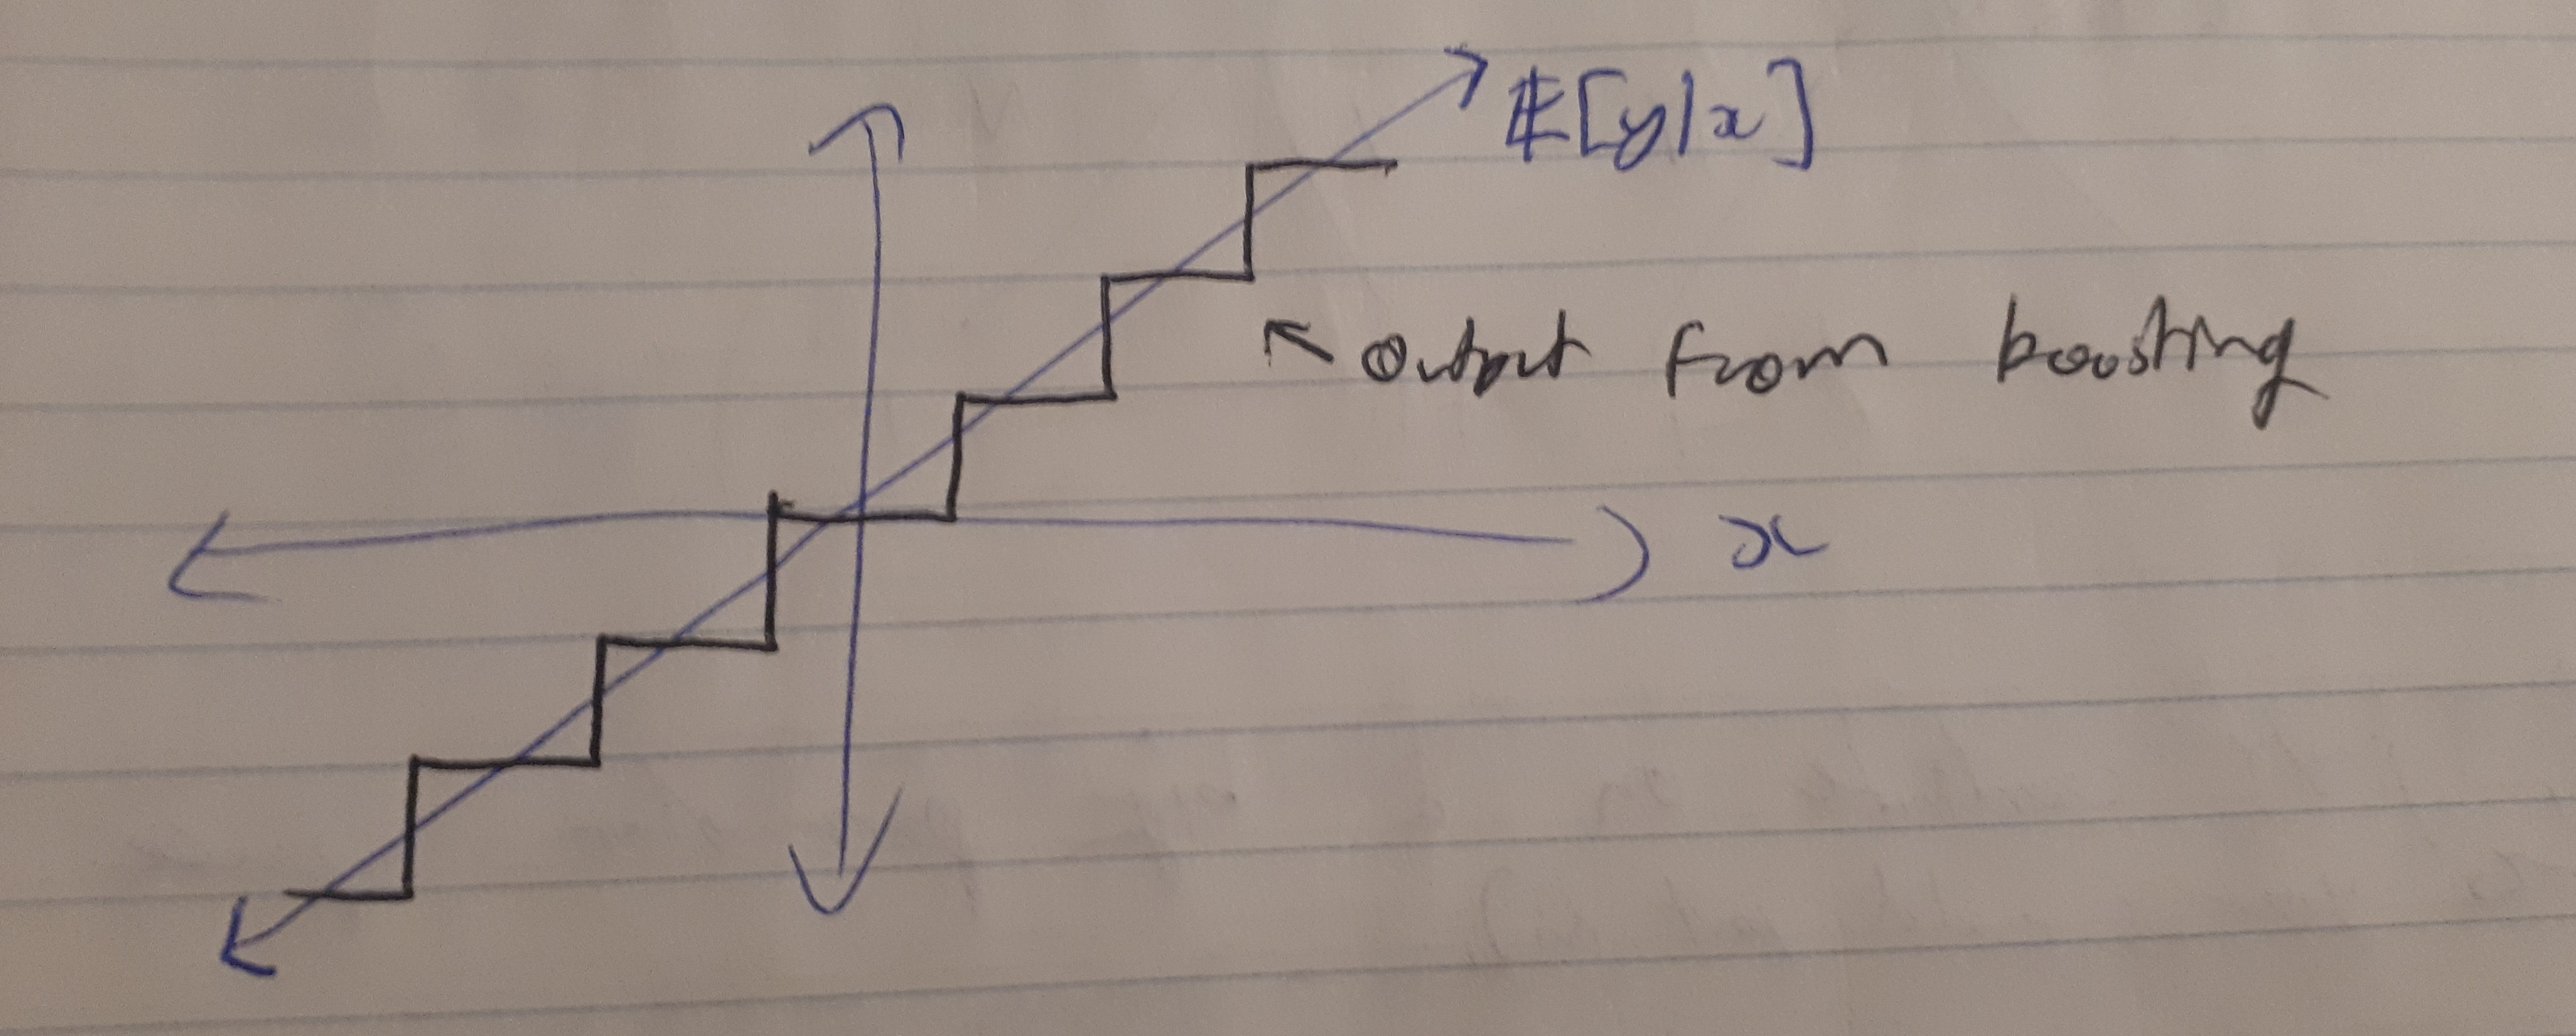
\includegraphics[width = 0.7\textwidth]{11_11_P02.jpg}
    \end{center}
    which is not very good. On the other hand if $\E[y|x]$ is non-linear, then boosting with decision trees works well. We would get results like this:\begin{center}
        
    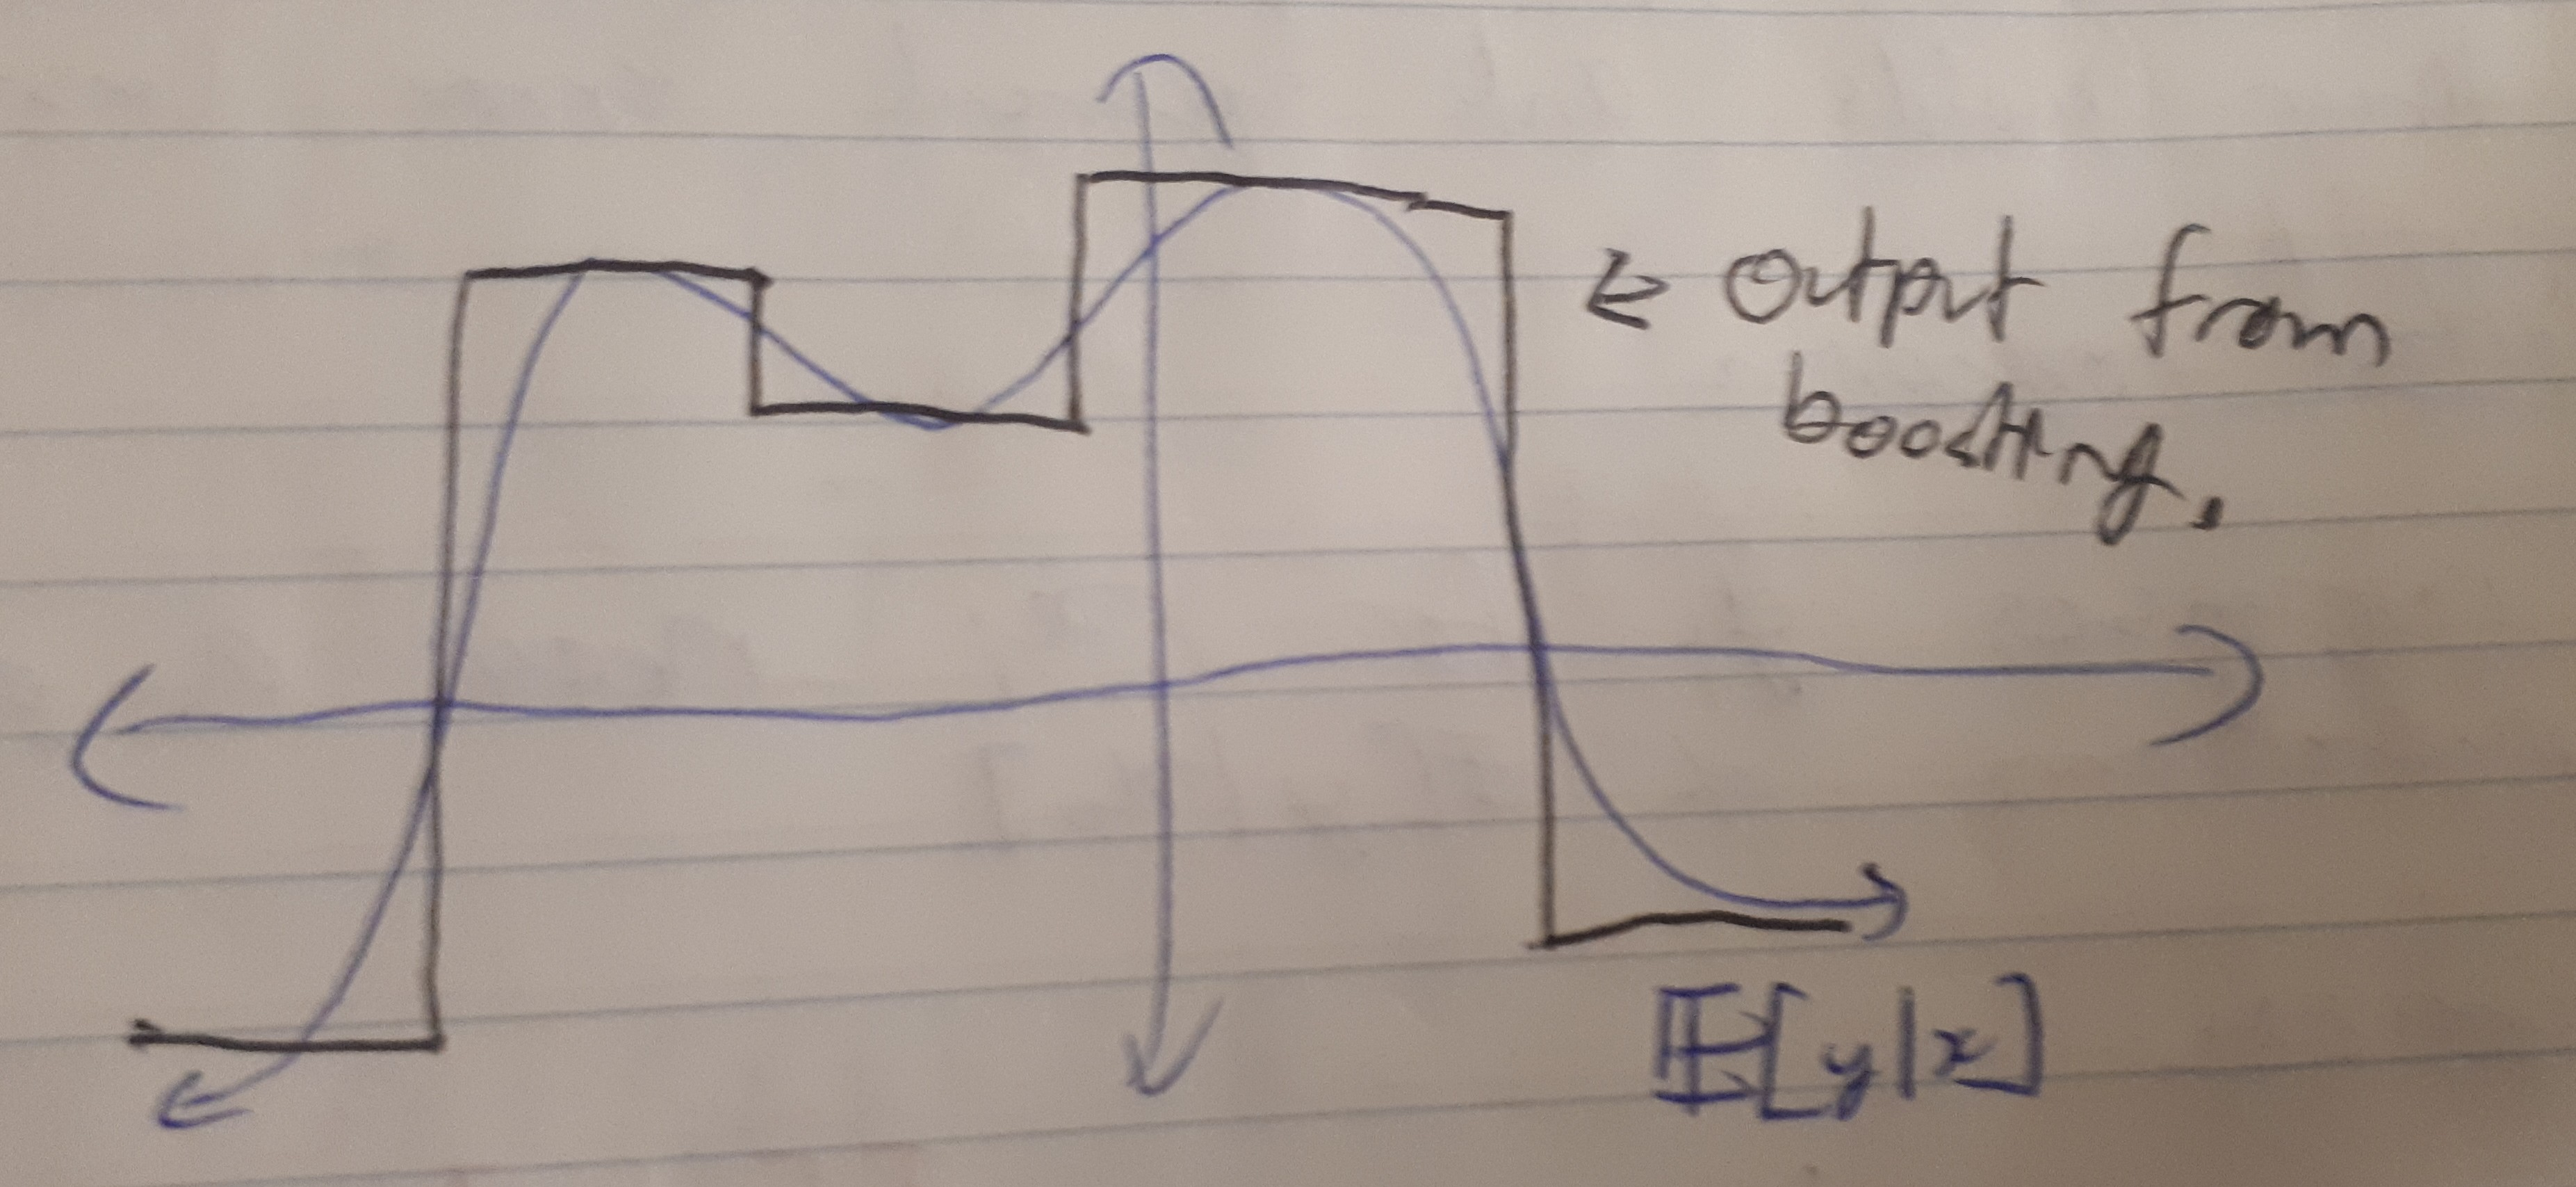
\includegraphics[width = 0.7\textwidth]{11_11_P03.jpg}
    \end{center}
    \item There isn't much understanding of the relationship between the strength of $\Phi$ and the final model.
    \item In partice we use cas use decision trees (or forests). For decision trees our weak learners are something like:
    \begin{center}
    
        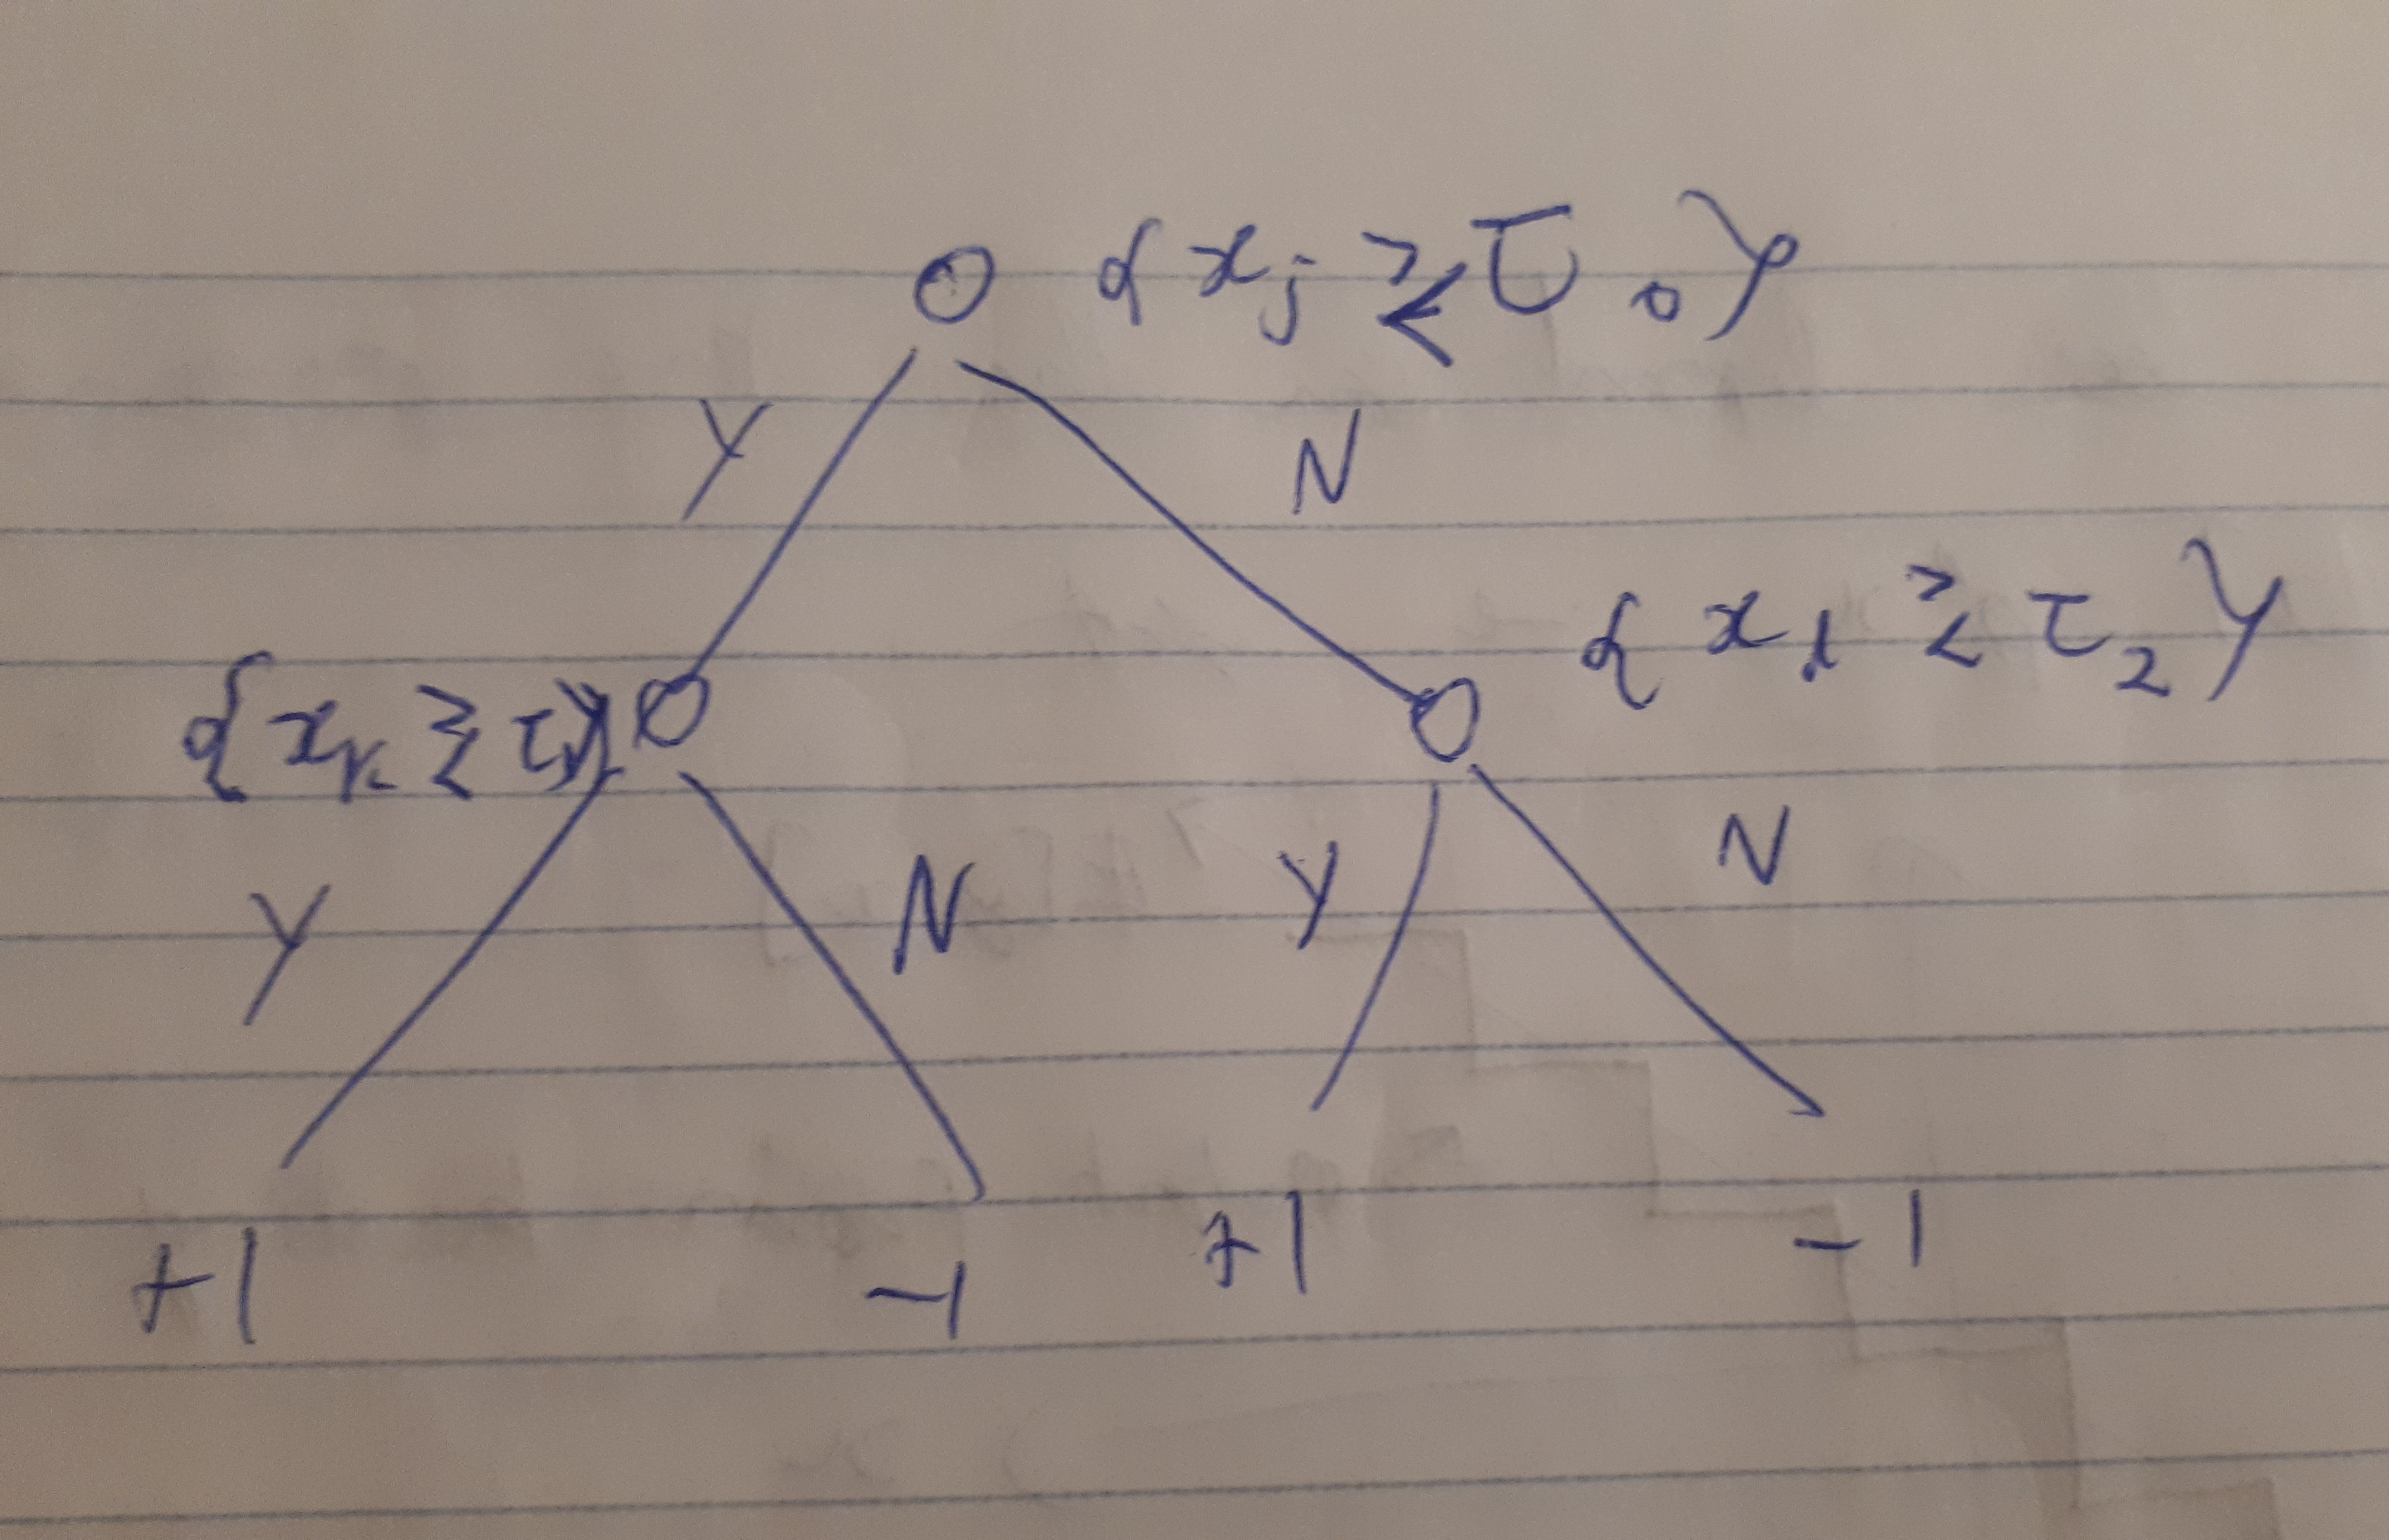
\includegraphics[width = 0.7\textwidth]{11_11_P04.jpg}    
    \end{center} 
    \item One perspective is that boosting is ``just'' coordinate descent on a very large parameter space.
    \item What we called \underline{version 1} is called \emph{gradient boosting} and is implemented in XG-Boost. What we called  \underline{version 2} doesn't really have a name. Version 2 does not generalize to other loss functions as well as version 1. It is just because we have linear models and square error that the calculations were possible.
\end{itemize}
\section{Locally weighted least squares}
Idea: use responses $y_i$ for $x_i$ near a given $x_0$ to make predictions of $\E[y|x_0]$. We want to predict $y$ at $x_0$ and we will use the idea that locally $\E[y|x]$ might be linear even if globally $\E[y|x]$ is non-linear. This would be the case if our looks something like this: 

\begin{center}
    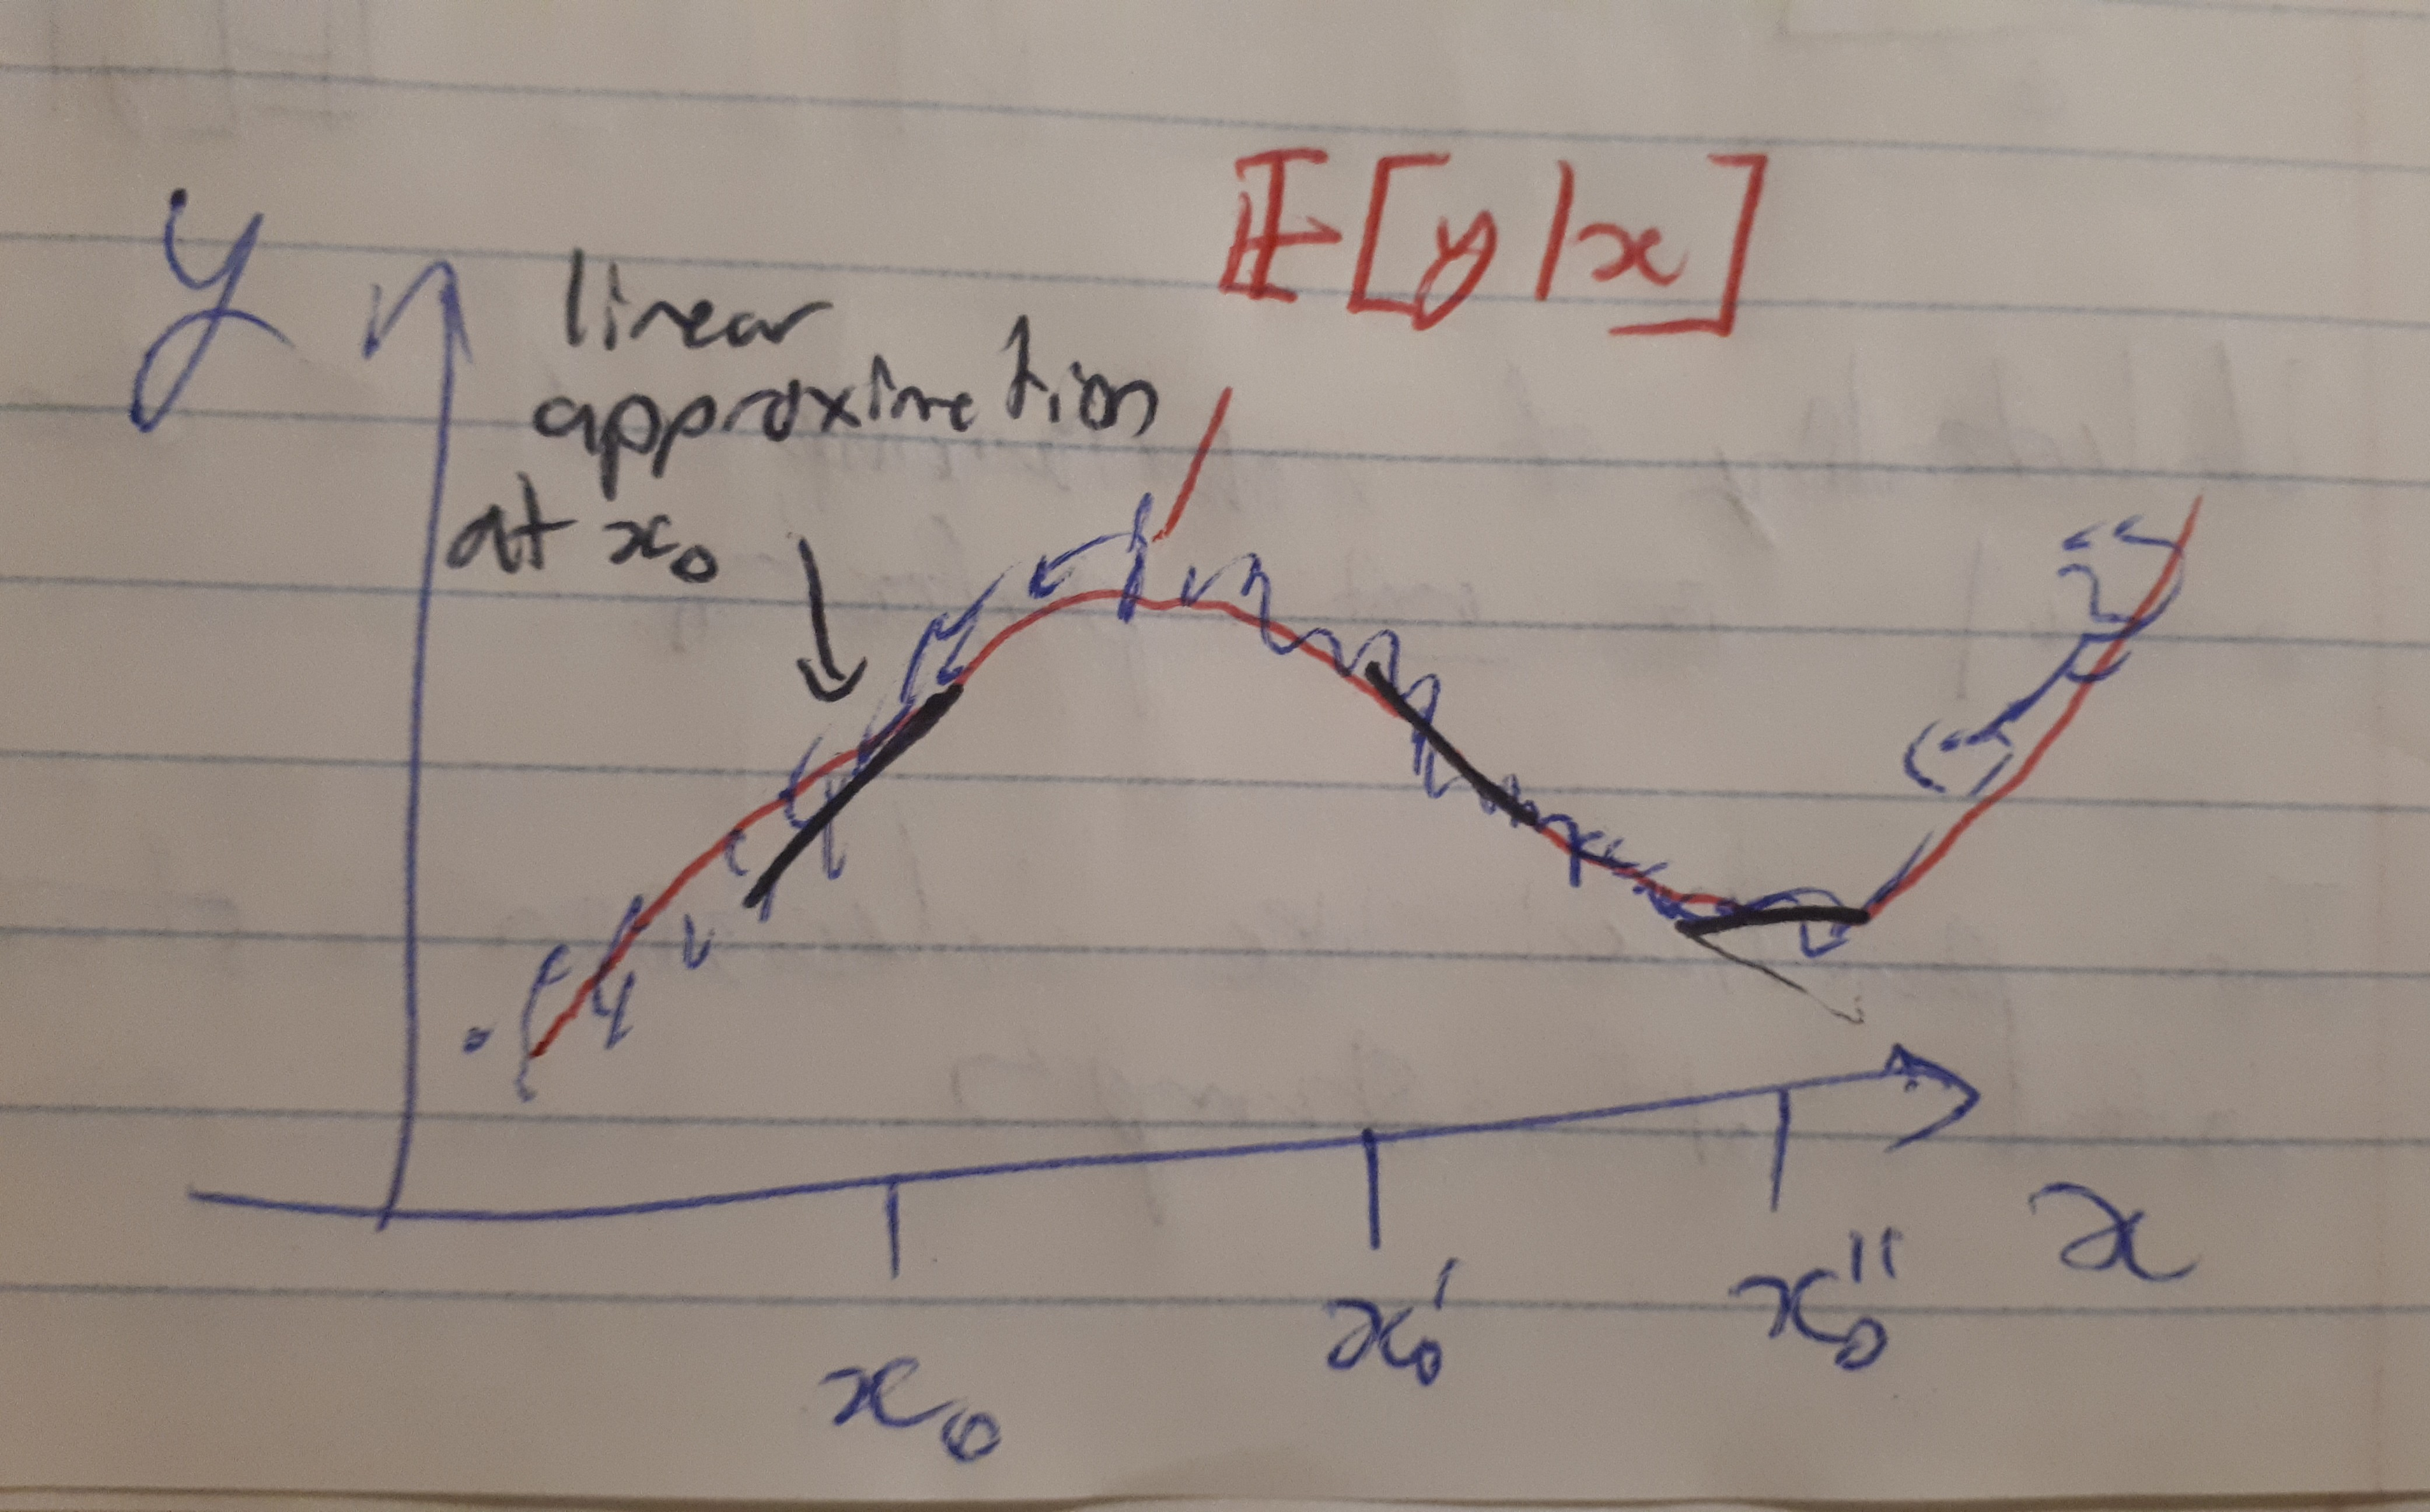
\includegraphics[width = 0.7\textwidth]{11_11_P05.jpg}    
\end{center}

Our prediction at $x_0 \in \R^d$ will be 
\[\wh{f}(x_0) = a_0+b_0^Tx_0,\]
where $(a_0,b_0)$ minimize
\[\sum_{i=1}^n W\left(\frac{\norm{x_i-x_0}^2_2}{\w}\right)(y_i-a-b^Tx_i)^2, \]
where $W : \R \to \R_+$ satisfies $W(0)=1$, $W(t) \le 1$ for $t \neq 0$. For example maybe $W(t) =\exp(-\frac{1}{2}t^2)$ or $W(t) = (1-\abs{t})^2_+$. In general $W(t)$ is some sort of function with a bump at 0 that goes to zero away from 0. The parameter $\w$ is called a bandwidth parameter.
\subsection{Fitting and predicting}
Suppose we want to make a prediction at $x_0$. Define $D(x_0)=\diag\left(W\left(\frac{\norm{x_0-x_i}_2^2}{\w}\right)\right) \in \R^{n\times n}$. Also define $Z=[1,X]$ where 
\[X=\begin{bmatrix}
    x_1\\\vdots \\ x_n
\end{bmatrix}, \]
Let $\ta = \begin{bmatrix}a\\ b\end{bmatrix} \in \R^{1+d}$, then
\begin{align*}
    \wh{\ta} &= \amin_\ta (y-Z\ta)^T D(x_0)(y-Z\ta)\\
    &= (Z^TD(x_0)Z)^{-1}Z^TD(x_0)y.
\end{align*}
Our prediction at $x_0$ is thus
\[\wh{f}(x_0) = \begin{bmatrix}1\\x_0\end{bmatrix}^T \wh{\ta} =\begin{bmatrix}1\\x_0\end{bmatrix}^T (Z^TD(x_0)Z)^{-1}Z^TD(x_0)y. \]
Note, that for predicting at $x_i$ we have 
\[\wh{y}_i = w(x_i)^T y, \]
where 
\[w(x_i) = D(x_i)Z(Z^TD(x_i)Z)^{-1}\begin{bmatrix}
    1\\x_i
\end{bmatrix}.\]
Thus $\wh{y} = Hy$ where 
\[H = \begin{bmatrix}
    w(x_1)^T\\
    \vdots \\
    w(x_n)^T
\end{bmatrix}.\]
The matrix $H$ is symmetric but does not satisfy $H^2=H$ so $H$ is not a projection matrix. But, since $\wh{y}=Hy$ is linear in $y$ all of our theory on $\E[\norm{\wh{y}-y}_2^2]$ still goes through.
\end{document}